\chapter{Background}
\label{ch2_background}
\section{What is Hardware Acceleration?}
\label{sect2_1}
Migration of some applications running on a general purpose CPU, to custom hardware acceleration engines, to resolve inherent bottlenecks of the system and improve system performance is referred to as hardware acceleration \cite{wiki_hwacc}. Such specialized accelerators intend to improve portions of the code that incur significant performance overheads such as:
\begin{itemize}
\item Mathematically rigorous functions with more data dependence and reduced control dependence among operations,
\item Repeated routines on different data sets,
\item Other parallelizable tasks, etc. 
\end{itemize}
Some common real-world scenarios demanding the computation bandwidth of hardware accelerators are Audio codec applications, high-speed Video Streaming, Network protocols, Cryptanalysis, Data mining, Natural Language Processing, Computer Vision, etc. \cite{ibm_devworks} The goal is to accomplish a faster execution time in hardware than in software. The hardware execution time includes the actual computation time by the accelerator as well as the communication overheads associated with reading and writing back the data. 

\section{Heterogeneous Platforms}
\label{sect2_2}
Heterogeneous computing platform constitutes different kinds of processors on the same silicon die. Commonly found constituents of an embedded system platform are a general-purpose processor (CPU) and a few specialized co-processors designed for a specific purpose. Examples of co-processors are Digital Signal Processors, which provide Instruction Level parallelism with VLIW, SIMD and superscalar capabilities, GPGPUs and FPGAs. The heterogeneous devices that were used for this project are listed below:
\subsection{Intel Platform with CPU and GPU}
This platform has been chosen to demonstrate code portability across different compute elements, evaluate the runtime of an application in CPU and GPU, analyze whether the given application is control-bound or compute-bound, and estimate the percentage improvement in latency. The \textbf{Intel SDK for OpenCL}\cite{intel_openclSDK} is available for both Windows and Linux Operating Systems and offers packages to run applications on Intel CPU and GPU. Also, the \textbf{OpenCL Runtime Environment} (RTE) \cite{intel_runtime} provides drivers and library packages required to test applications while they are running. The installation of these packages will be discussed in detail in Section \ref{3_1_3_1}.   
\subsection{Avnet Zedboard with Xilinx Zynq 7000\\All-programmable SoC}
This platform comprises of a Processing System with dual-core ARM Cortex A9, running at 667 MHz with NEON SIMD engine and Floating Point Unit, and a Programmable Logic with Artix-7 FPGA. The processing system and programmable logic are connected via AXI Interface. Zedboard has found its place in different market segments, be it Automotive, Consumer Electronics, software-defined Radio applications \cite{dobson2014architecture}, Aerospace and Defense, Medical diagnostics and Imaging, Wired and Wireless communication, Control and Bridging applications \cite{xil_zynqbrief}. Owing to its versatility, this platform has been chosen to conduct experiments on the complex applications at hand.
\section{Programming Models for Hardware Acceleration}
\label{2_3}
The various programming models that have been explored in this thesis are discussed below. The models have been chosen with the view to reducing the burden on the engineers to learn coding at lower levels of abstraction while also achieving unparalleled performance.
\subsection{GPGPUs}
\label{2_3_1}
The first half of this thesis delves into the use of GPGPUs for applications other than their conventional role in computer graphics. The most commonly used programming languages for GPU programming are Open Computing Language (OpenCL) and CUDA. It is interesting to note that CUDA implementations currently support only one vendor, NVIDIA Corporation while OpenCL supports the vendors AMD, Intel, Altera, NVIDIA and Apple.\newline \newline
While OpenCL is open-source, CUDA is proprietary. After a basic run-through of the features of both frameworks such as code portability and flexibility, OpenCL programming model was chosen to carry out the acceleration experiments. The prime focus of this thesis is on OpenCL C APIs, which are maintained by the Khronos group \cite{khronos2008opencl}. The OpenCL architecture is composed of a Host which dispatches commands to the devices. The host CPU offsets loads to the devices and the devices execute these workloads for the host.

\begin{figure}[h!]
  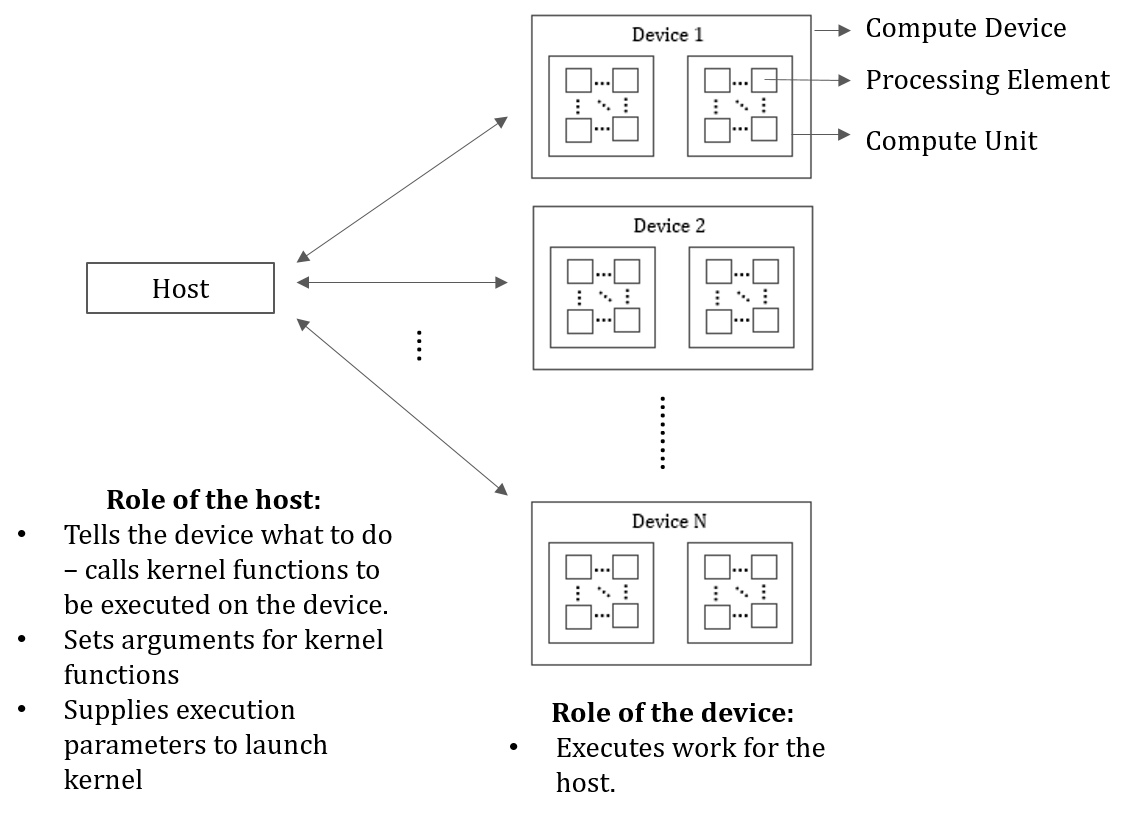
\includegraphics[width=\linewidth]{figures/openCL_architcture.png}
  \caption{The OpenCL Platform Model
  \cite{rosenberg2011opencl}}
  \label{fig:openCL_architecture}
\end{figure}

There are three popular OpenCL Models \cite{opencl_ajg}, which shall be discussed briefly to aid the understanding of internals in OpenCL Programming. 
\subsubsection{Device Model}
\label{2_3_1_1}
It is an abstract view of various components in a Compute device. 
Each device consists of various Compute Units, and each of those compute units are composed of several Processing Elements (PEs). 
Hence, Compute units can be viewed as containers of very simple processors (PEs). 

\begin{figure}[h!]
  \centering
  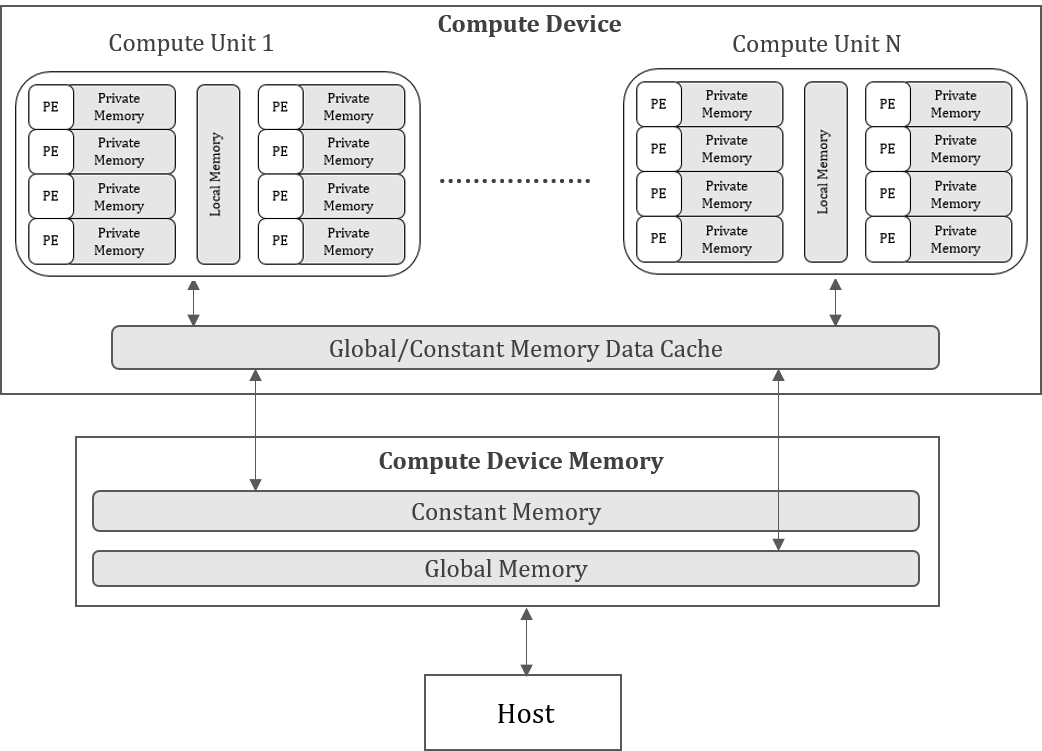
\includegraphics[width=0.80\linewidth]{figures/openCL_deviceModel.png}
  \caption{The Device Model of OpenCL
  \cite{opencl_ajg}}
  \label{fig:openCL_deviceModel}
\end{figure}

\subsubsection{Memory Model}
\label{2_3_1_2}
It defines the memory hierarchy inside an OpenCL device. 
\begin{itemize}
\item \textbf{Global Memory:} Persistent storage accessible by all Processing Elements (PEs) and the host.
\item \textbf{Constant Memory:} Non-persistent, Read-Only Memory shared among all Processing Elements.
\item \textbf{Local Memory:} Shared by all PEs in one Compute Unit and not available to PEs from other compute units. Each Compute Unit has its own local memory.
\item \textbf{Private Memory:} Non-persistent memory accessible by a single Processing Element.
\end{itemize}
\subsubsection{Execution Model}
\label{2_3_1_3}
OpenCL \textbf{kernels} are ordinary functions with special signatures written in OpenCL C, which run on each Processing Element. For data-parallel applications where the same function is invoked several times, the kernels execute in parallel on different PEs over a pre-defined N-dimensional index space \cite{tompson2012introduction}. \newline \newline
A \textbf{work item} is an independent element of execution. It can also be interpreted as the invocation of the kernel for a specific index “i”. The \textbf{global work size} defines the number of work items per work dimension (dimension of the index space).\newline \newline
The host describes an N-dimensional computational load where each index point is represented by a work item. The work items are grouped into \textbf{work groups} by the host and each of these work groups execute in parallel within the compute unit. The work group size is device-dependent and can be found by querying the device using OpenCL APIs. 
Each Compute Unit has its own work-group(s) and each work item in the work group is executed by a single processing element.

\begin{figure}[h!]
  \centering
  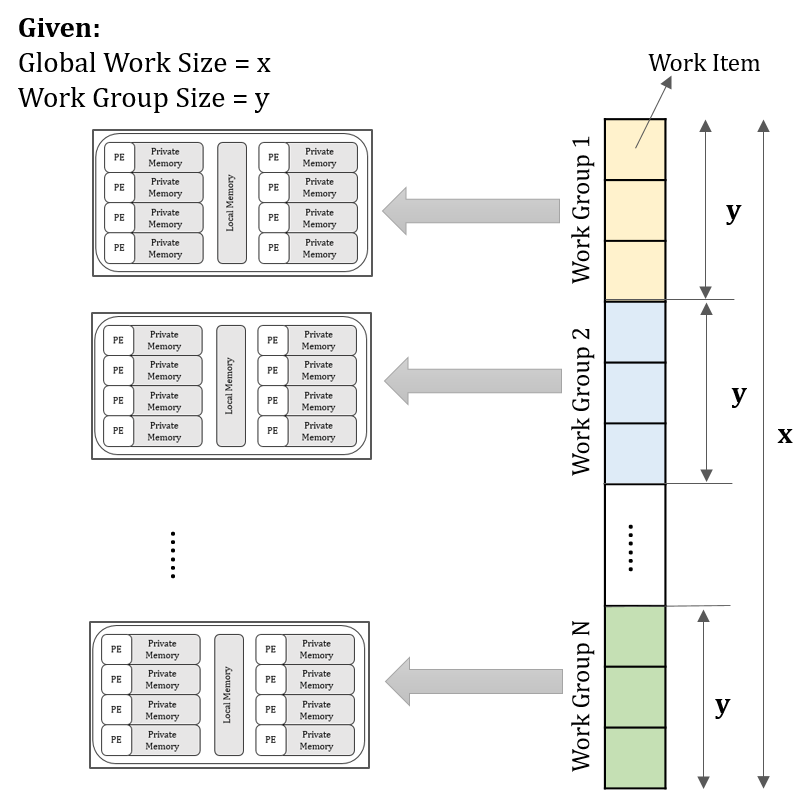
\includegraphics[width=0.70\linewidth]{figures/openCL_workSchedule.png}
  \caption{An Illustration of Data-parallel execution
  \cite{opencl_ajg}}
  \label{fig:openCL_workSchedule}
\end{figure}

\subsection{Field Programmable Gate Arrays}
\label{2_3_2}
\subsubsection{High-Level Synthesis}
\label{2_3_2_1}
Until recently, we were directing our attention to programming in specialized processors using high-level languages such as C and C++. With growing computational demand, a sudden shift in focus to FPGAs necessitated the hardware programming knowledge among software engineers. \newline \newline
The Figure \ref{fig:graph-rtldesign} depicts implementation time for various programming models and we notice that RTL design, although the most beneficial in terms of performance compared to standard and specialized processors, demands the highest development time, beyond the acceptable software development time, to capture the market. This can be attributed to the increased concretization in the design at lower-levels and the deficit of hardware programming experience and expertise.
\begin{figure}[h!]
  \centering
  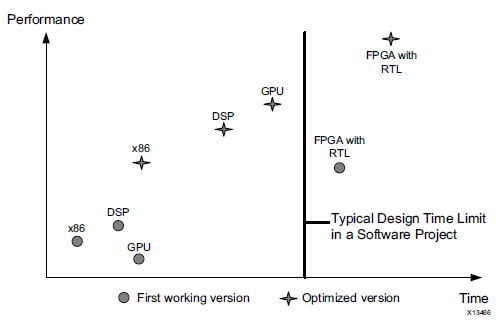
\includegraphics[width=0.8\linewidth]{figures/graph-rtldesign.png}
  \caption{Performance vs. Design Time with RTL Design
  \cite{xil_hls}}
  \label{fig:graph-rtldesign}
\end{figure}
To relieve the engineers of this burden and improve the time-to-market, High-Level Synthesis tools which eliminate the differences in programming models of processors and FPGAs have been introduced. HLS tools translate a C/C++ specification into an equivalent RTL description. The Figure \ref{fig:graph-hlsdesign} illustrates the performance peaks that can be accomplished with High-Level Synthesis, in comparison to standard processors and GPUs. 
\begin{figure}[h!]
  \centering
  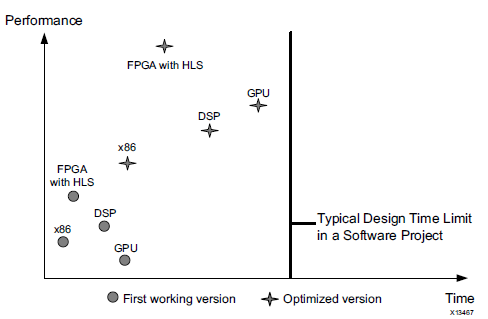
\includegraphics[width=0.8\linewidth]{figures/graph-hlsdesign.png}
  \caption{Performance vs. Design Time with HLS Compiler
  \cite{xil_hls}}
  \label{fig:graph-hlsdesign}
\end{figure}
It is only fair that we acknowledge the fact that RTL code automatically generated by HLS tools may not be the most optimal implementation. It may not fully exploit the parallelism offered by the underlying hardware, unlike the design with HDL languages. However, it meets the time limit specified for software development in many cases and hence proves very useful in that respect.\newline \newline 
Pointers are supported in HLS when they can be completely described at compile-time, without any need for runtime intelligence. FPGA-based designs using HLS demand the data and size of memory blocks to be deterministic at compile-time. This static memory allocation facilitates realization of an algorithm’s memory as a register, FIFO or Block RAM \cite{xil_hls}. \newline \newline
Register-based memory implementation is the fastest as a register is an independent entity, which doesn’t require any addressing logic. FIFOs are used to transfer data between loops and functions. It is a queue with a single entry and exit point. FPGAs have dedicated Random-access memory blocks called Block RAMs which retain values for as long as the system is powered on. Block RAMs support parallel access of two different memory locations. \newline \newline
HLS tools provide easy testing of functional correctness in both C and RTL implementations and offer numerous optimization directives, which when aptly used, help accomplish multi-objective optimizations.
\subsubsection{OpenCL}
\label{2_3_2_2}
OpenCL standard facilitates implementing parallel algorithms at higher levels of abstraction on FPGAs as opposed to traditional low-level programming using Hardware Description Languages such as VHDL and Verilog \cite{opencl_vhblog}. The drawbacks of High-level Synthesis tools in this respect is that they take in a sequential C description and try to extract thread-level parallelism out of it. Failure to gain the maximum parallelism beats the purpose of using an FPGA. Thus, OpenCL standard allows spawning of threads and annotating them with explicit constructs that describe parallelism and memory access hierarchy (execution parameters discussed in Figure \ref{fig:openCL_architecture}).\newline \newline
Unlike the CPU-GPU platform where concurrent threads are run on different cores, kernels are translated to equivalent dedicated circuits which implement each function in the hardware. These circuits are wired appropriately to simulate the dataflow in the kernel \cite{singh2011implementing}. The final circuit implemented on FPGAs is heavily pipelined and exhibits multi-threading capabilities, offering a final design with pipelined parallelism.\newline \newline
In conventional RTL design, the designers should handle cycle-wise hardware descriptions, create data paths, create FSMs for control flow, manage timing constraints and integrate low-level IP cores to the design, all by themselves. OpenCL Compiler automates these steps and helps shift the focus to refining the algorithm rather that detailing the hardware design. OpenCL being a cross-platform standard can be easily carried forward to different FPGA generations with little design effort, while the benefits of improved capabilities and performance remain intact \cite{singh2011implementing}.
\begin{figure}[h!]
  \centering
  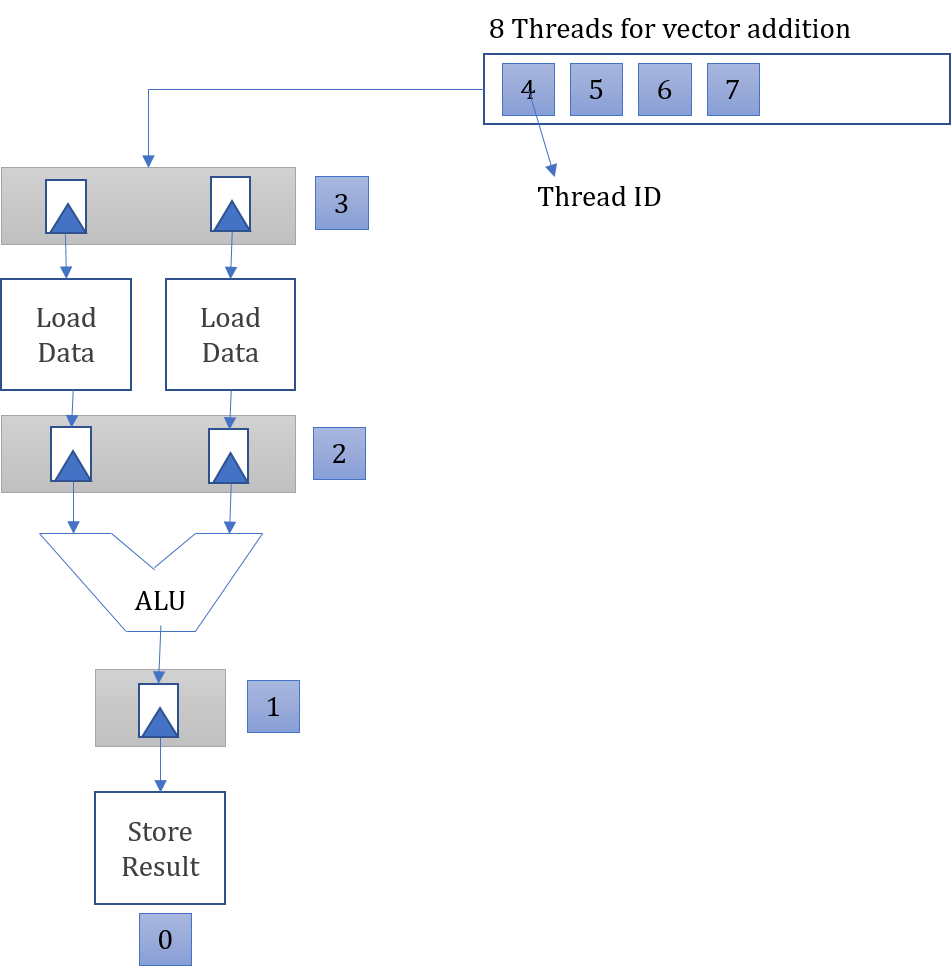
\includegraphics[width=0.6\linewidth]{figures/pipelined_parallelism_fpga_opencl.png}
  \caption{Pipeline Parallelism achieved by OpenCL-to-FPGA compiler
  \cite{singh2011implementing}}
  \label{fig:pipeline_parallelism_fpga_opencl}
\end{figure}
Figure \ref{fig:pipeline_parallelism_fpga_opencl} depicts the pipelined execution of the 8 threads by the generated circuit. Assuming there are three pipeline stages, at cycle 3, we observe that thread 0 stores the computed result, thread 1 computes the sum for a new set of data values, thread 2 copies the values read from memory while thread 3 reads data from the memory. Thus, at any point during the execution, all pipeline stages manipulate a different thread and all stages of the pipeline are active, until the processing of all threads are complete. \newline \newline
Some FPGA vendors like Xilinx and Altera offer OpenCL SDKs for FPGAs. We are not using the Altera Toolchain for our experiments, but the benchmark code taken for test relies on some platform-independent C++ headers (aocl\_utils) and Quartus II Emulator that are available with this SDK. Hence, this thesis shall make use of Altera OpenCL (AOCL) SDK to analyze and modify the code and study the results.
